\documentclass[pdflatex]{article}
\usepackage[frenchb]{babel}
\usepackage[T1]{fontenc}
\usepackage[latin1]{inputenc}
\usepackage{varioref}
\usepackage{graphicx}
\usepackage[left=2cm,top=1cm,right=2cm,nohead,nofoot]{geometry}

\begin{document}

\title{Visual R reference card (Draft)}

\maketitle

\author Sylvain Loiseau <sylvain.loiseau@unicaen.fr>

Universit\'e de Caen--Basse Normandie

\section{Graphical conventions}
% ----------------------------

In this document, evaluations of R expressions are represented graphically. For
instance, the expression "c(7, 5) + 3", which create a vector and add 3 to
its elements, is represented as follow:

\begin{tabular}{c}
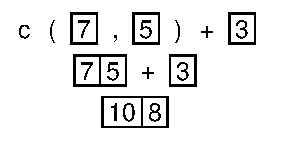
\includegraphics{graphical_conventions}
\end{tabular}

The first line represent the expression you typed in, the last line give the
object eventually created, and each intermediary line is a step in the
evaluation of the expression.

\section{Anatomy of a vector}
% ----------------------------

All elements of a vector have a common mode, one of character, logical, and numeric.

\begin{tabular}{ccc}
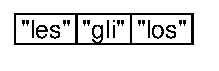
\includegraphics{v_char} & 
\includegraphics{v_log} & 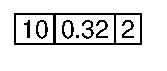
\includegraphics{v_num}\\
\end{tabular}

All elements of a vector have an index. They may have a name.

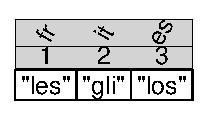
\includegraphics{v_char_names} 

All vectors have two important properties : their mode and their length.

\begin{tabular}{cc}
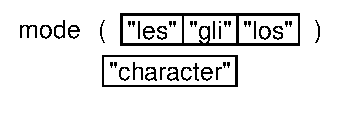
\includegraphics{v_char_type} & 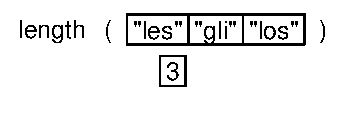
\includegraphics{v_char_length}\\
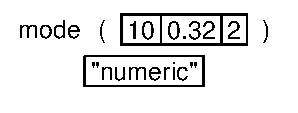
\includegraphics{v_num_type} & 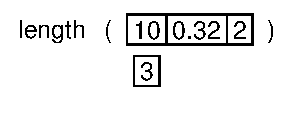
\includegraphics{v_num_length}\\
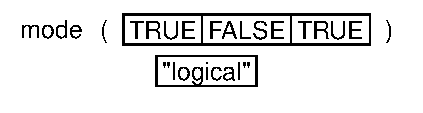
\includegraphics{v_log_type} & 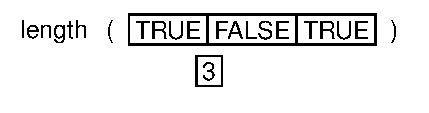
\includegraphics{v_log_length}\\
\end{tabular}

Functions are precisly defined in terms of mode, number and length of vectors they may take as argument, and mode and length of vector they create.

\begin{enumerate}
\item length() take one vector of any mode and length and return a vector of numeric vector of length 1.
\item mode() take one vector of any mode and length and return a character vector of length 1.
\end{enumerate}

\section{Creating a vector}
% ----------------------------

\begin{tabular}{cc}
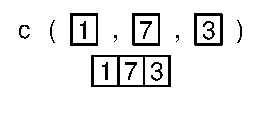
\includegraphics{c_1} & 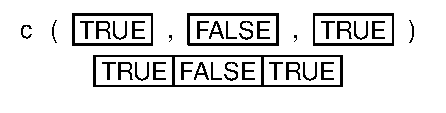
\includegraphics{c_2}\\
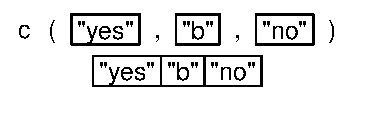
\includegraphics{c_3} & \\
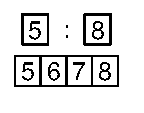
\includegraphics{operator_sequence} & 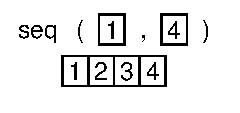
\includegraphics{seq}\\
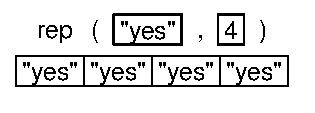
\includegraphics{rep} & 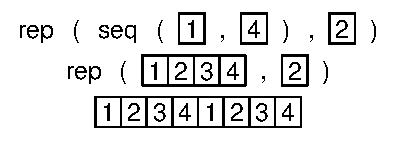
\includegraphics{rep_seq}\\
\end{tabular}

The function c() take any number of vectors of any length and any mode, but all vectors must have the same mode (see below, "Conversion"). It returns a vector of the same mode as the arguments and whose length is the sum of the length of its arguments.

\section{Extraction}
% ----------------------------

A vector can be created by extracting some elements of a vector.

Elements to be extracted can be addressed using their index.

\begin{tabular}{cc}
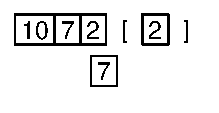
\includegraphics{extract_num} 
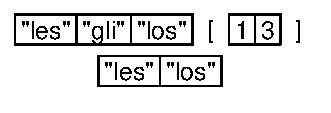
\includegraphics{extract_nums} 
\end{tabular}

Index are 1-based. If an index is greater than the number of element in the vector, you get "NA". If the vector has names, their are preserved.

\begin{tabular}{cc}
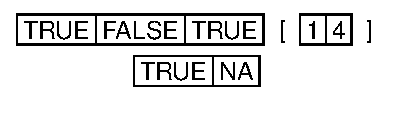
\includegraphics{extract_nums_outsider} & 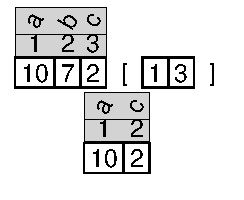
\includegraphics{extract_nums_names}
\end{tabular}

You can also extract with character or logical vector inside the square brackets of the extraction operator. Elements of a character vector are interpreted as the names of the elements to be extracted (elements must have names!).

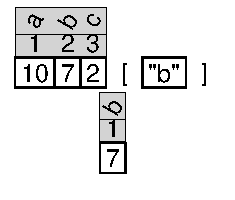
\includegraphics{extract_char_names}

Logical vectors must have the same length as the vector to be extracted. Elements are extracted if there is a "TRUE" value at the same position in the logical vector. (If the logical vector is shorter, it is recycled: right (see below for recycling))

\begin{tabular}{ll}
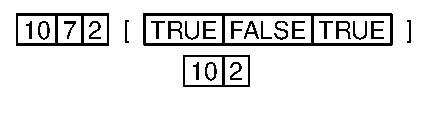
\includegraphics{extract_logical} & 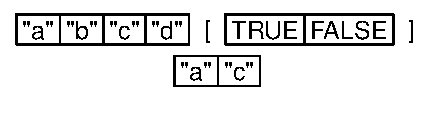
\includegraphics{extract_logical_recycling}\\
\end{tabular}

When extracting, nothing prevent you from reordering elements or extracting  several times the same element:

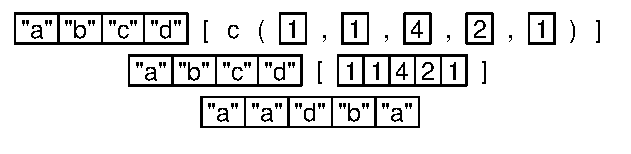
\includegraphics{extract_repeating}

\section{Operator}
% ----------------------------

Some numeric operators.

\begin{tabular}{ccc}
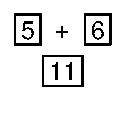
\includegraphics{operator_plus} & 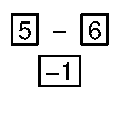
\includegraphics{operator_minus} & 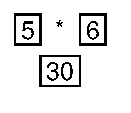
\includegraphics{operator_time}\\
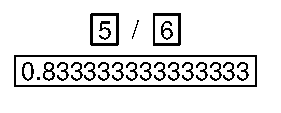
\includegraphics{operator_div} & 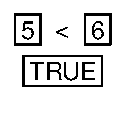
\includegraphics{operator_strict_lt} & 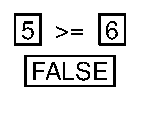
\includegraphics{operator_gt_or_equal}\\
\end{tabular}

Some logical operators.

\begin{tabular}{ccc}
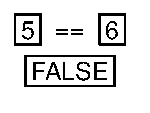
\includegraphics{operator_equality_num} & 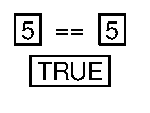
\includegraphics{operator_equality_num_TRUE}\\
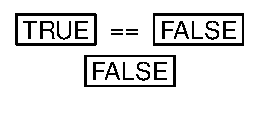
\includegraphics{operator_equality_log} & 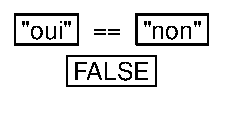
\includegraphics{operator_equality_char}\\
\end{tabular}

\section{Vectorization}
% ----------------------------

Operators -- as well as many functions -- may operate on vector of any length: the operation is performed on pair of elements of equal index.

\begin{tabular}{cc}
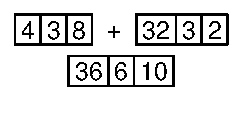
\includegraphics{operator_plus_vectorized} & 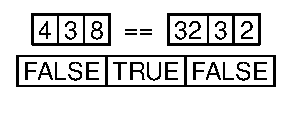
\includegraphics{operator_equal_vectorized}\\
\end{tabular}

\section{Recycling}
% ----------------------------

In a context where vectorization is allowed, you may provide vectors of unequal length. The shorter is duplicated until its length reach the length of the longer. This is called recycling a vector.

\begin{tabular}{cc}
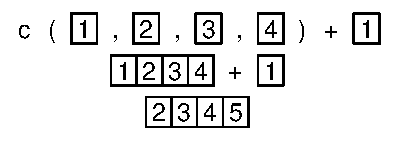
\includegraphics{operator_add} & 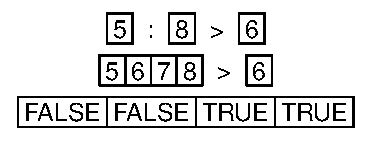
\includegraphics{operator_gt}\\
\end{tabular}

There is no need to express a loop in order to add 1 to all elements of a
vector.

Be careful:

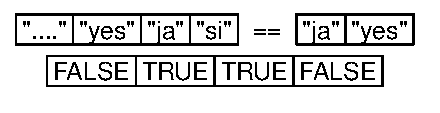
\includegraphics{operator_recycling}

\section{Some numeric functions}
% ----------------------------

Some functions for numeric vectors.

\begin{tabular}{cc}
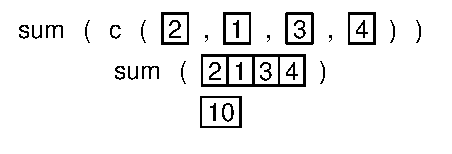
\includegraphics{sum} & 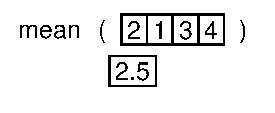
\includegraphics{mean}\\
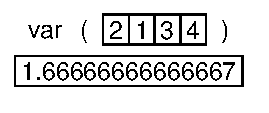
\includegraphics{var} & 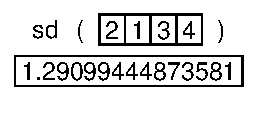
\includegraphics{sd}\\
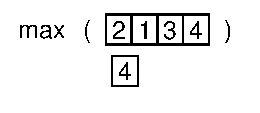
\includegraphics{max} & 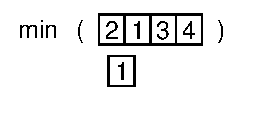
\includegraphics{min}\\
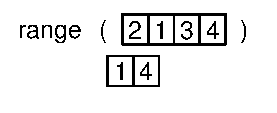
\includegraphics{range} & \\
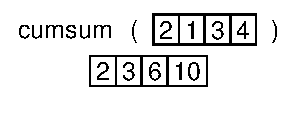
\includegraphics{cumsum} & 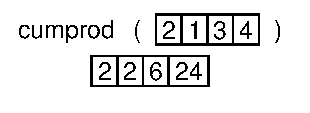
\includegraphics{cumprod}
\end{tabular}

%\includegraphics{crossprod}

\section{Some string functions}
% ----------------------------

nchar() count the number of characters in all strings of a character vector.

\includegraphics{nchar}

Recycling and vectorization are useful with paste(), which concatenates characters string at same index in several characters vectors:

\begin{tabular}{cc}
\includegraphics{paste} & \includegraphics{paste2}\\
\includegraphics{paste3} & \includegraphics{paste4}\\
\end{tabular}

You can paste more than two vectors of characters:

\includegraphics{paste5}

\section{Sorting}
% ----------------------------

Numeric and character vectors can be sorted. Names are preserved.

\begin{tabular}{cc}
\includegraphics{sort} & \includegraphics{sort2}\\
\includegraphics{sort_char} & \includegraphics{sort_char_names} \\
\end{tabular}

Flipping a vector:

\includegraphics{rev}

\section{Type conversion}
% ----------------------------

c() coerce its arguments to a common mode -- all elements of a vector always
have a common mode.

The character mode always wins. Logical always looses.

\begin{tabular}{cc}
\includegraphics{conversion_1} & \includegraphics{conversion}\\
\end{tabular}

Many functions silently convert their arguments to the requiered mode. For
instance, the function nchar() give the number of characters of the elements of
a character vector. It makes sense only for characters string: numbers don't
have a "number of characters" themselves, but inside a convention of
representation as characters strings. If the function nchar() receive a vector
of another mode (numerical, logical), the vector is silently converted into a
characters vector using as.character() (left). The result is identical to
explicitly converting into characters, using as.character() (right).

\begin{tabular}{cc}
\includegraphics{conversion_nchar} & \includegraphics{conversion_as_character}\\
\end{tabular}

\section{Index}
% ----------------------------

Some useful functions give index rather than the actual values.

\includegraphics{which}

\begin{tabular}{cc}
\includegraphics{order} & \includegraphics{order2}\\
\includegraphics{which_min} & \includegraphics{which_max}\\
\end{tabular}

This is particularly usefull in very common situations where two or more
vectors are "aligned", or "synchronized". Suppose two vectors: a character
vector giving forms in a corpus (left), and a numeric vector giving the total
frequency for each form (right):

\begin{tabular}{cc}
\includegraphics{v_forms} & \includegraphics{v_frequencies}\\
\end{tabular}

Using max(), you may retrieve the maximum frequency from the second vector, but
you can't figure out which form have this frequency. Using which.max(), you're
still able to extract the corresponding value in the first vector:

\begin{tabular}{c}
\includegraphics{which_max_2}
\end{tabular}

Again, suppose you want to sort the row of a matrix according to the value in a
column. You cannot use sort, since it give the actual values sorted, not the
index of the row sorted. Order is commonly used for reordering data structure:

\begin{tabular}{c}
\includegraphics{matrix_order}
\end{tabular}

\section{Precedence}
% ----------------------------

Operators have precedence (see ?Syntax).

"seq" takes precedence over "+", "seq" takes precedence over logical operators...

\begin{tabular}{cc}
\includegraphics{precedence} & \includegraphics{operator_gt}\\
\end{tabular}

The order in which the operators are written in the code does not matter!

\includegraphics{operator_gt_inv}

\section{Matrix}
% ----------------------------

\subsection{Creation}

Matrix are created with the matrix() function. It takes three main arguments: a
vector (any mode and any length) gives the content, two vectors (numeric and
length 1) give the numbers of rows and columns. If only one dimension is given,
the second one is deduced from the length of the vector. If both dimensions are
given and the vector length do not match the number of cells, the vector is
recycled to fill the matrix. The matrix is filled by column; this behavior may
be changed with the option byrow. 

\begin{tabular}{cc}
\includegraphics{matrix} & \includegraphics{matrix_arg}\\
\includegraphics{matrix_byrow} & \includegraphics{matrix_nbcol}\\
\includegraphics{matrix_logical} &
\end{tabular}

\subsection{Extraction with a matrix}

Matrices have two dimensions and you must provide extractors for each of them.
You first extract the rows, then the columns.

\begin{tabular}{cc}
\includegraphics{matrix_extraction} & \includegraphics{matrix_extraction3}\\
\includegraphics{matrix_extraction2} & \includegraphics{matrix_extraction4}\\
\end{tabular}

%\begin{tabular}{cc}
\includegraphics{matrix_extraction5}
%& \includegraphics{matrix_extraction_drop}
%\end{tabular}

If you leave blank the column slot, all columns are selected (left); if you leave blank the row slot, all rows are selected (right).

\begin{tabular}{cc}
\includegraphics{matrix_extraction_rows} & \includegraphics{matrix_extraction_columns}\\
\end{tabular}

How does extraction in a matrix preserve names? No name is preserved if you extract a single element; longuest dimension's names are preserved if you extract a vector of more than one element, both dimensions are preserved if you extract a sub-matrix:

\includegraphics{matrix_extraction8}
\includegraphics{matrix_extraction6}
\includegraphics{matrix_extraction7}

\subsection{Properties}

\begin{tabular}{ccc}
\includegraphics{nrow.pdf} & \includegraphics{ncol.pdf} & \includegraphics{dim.pdf}
\end{tabular}

\begin{tabular}{cc}
\includegraphics{rownames.pdf} & \includegraphics{colnames.pdf}
\end{tabular}

\begin{tabular}{cc}
\includegraphics{length_matrix.pdf} & \includegraphics{mode_matrix.pdf}
\end{tabular}

A matrix is very similar to a vector: it has a mode and a length. It has also
two dimensions and, then, it has two vector of names and it takes two index
vectors inside extraction operator. But you can often see a matrix as a vector.
For instance, if you use only one index vector inside the extraction operator,
it extracts from the underlying, column-filled vector:

\includegraphics{matrix_extraction_as_vector}

\subsection{Summing a matrix}

\includegraphics{matrix_sum} 

\begin{tabular}{ccc}
\includegraphics{rowSums} & \includegraphics{colSums}
\end{tabular}

\subsection{Changing}

\begin{tabular}{cc}
\includegraphics{as_vector} & \includegraphics{matrix_operator}\\
\end{tabular}

\begin{tabular}{cc}
\includegraphics{cbind.pdf} & \includegraphics{rbind.pdf}\\
\end{tabular}

\begin{tabular}{c}
\includegraphics{t.pdf}\\
\end{tabular}

\section{list}
% ----------------------------

\subsection{Creation, anatomy}

Creating a list by enumerating its components.

A list of length 4: contains 4 vectors, each of length 1 (left) ;
a list of length 1: contains 1 vector of length 2 (right).

\begin{tabular}{cc}
\includegraphics{list_enumerate.pdf} & \includegraphics{list_onetype.pdf}
\end{tabular}

% Same as above
% 
% \includegraphics{list.pdf}

List can contain objects of different mode (left) ;
it can contain objects of different dimensions (right).

\begin{tabular}{cc}
\includegraphics{list_twotypes.pdf} & \includegraphics{list_matrix.pdf}
\end{tabular}

A list can be recursive: a component may be a list.

\includegraphics{list_complex.pdf}

% \includegraphics{list_rec.pdf}

\subsection{Basic functions}

\includegraphics{list_names}

\includegraphics{list_length}

\includegraphics{list_mode}

\subsection{Extraction}

Extracting in a list. The next two figures show the difference beween [ and [[ operator on list: the first create a sublist (it extracts elements, exactly as it extracts elements from a vector), while the second is completely different: it give the content of one (and only one) element of a list.

\begin{tabular}{cc}
\includegraphics{list_extract_simple.pdf} & \includegraphics{list_extract_double.pdf}
\end{tabular}

You can use vector of any length within the single-square bracket, while you can address only one element within the double-square-bracket operator, and then use only vector of length 1.

Since a list is a recursive data structure (may contain list), you can use several successive bracket operators in order to go down to the element you're interested in.

With the single-square-bracket operator you cannot walk down though the data structure.

\includegraphics{list_successive_extraction}

Be sure to understand the difference between "lengt(l[1])" and length(l[[1]])" :

\begin{tabular}{cc}
\includegraphics{list_extraction_1.pdf} & \includegraphics{list_extraction_2.pdf}
\end{tabular}

\subsection{List and vector}

\begin{tabular}{cc}
\includegraphics{unlist} & \includegraphics{aslist}
\end{tabular}

\subsection{List for expressing complex data structure}

List are useful for expressing complex data structure.

- Grouping elements of a vector using a the level of a factors (see Factor below and the function split())

- Splitting strings (See strsplit() below).

% \includegraphics{split}

\section{Factor}
% ----------------------------

A factor represent a nominal random variable. It looks like a character
vector, and may be created using a character vector (left). In this document,
factors are represented without quotes around the values. The different values in
the factor (the different modality in the random variable) may be retrieved
using levels() (right).

\begin{tabular}{cc}
\includegraphics{factor} & \includegraphics{levels}\\
\end{tabular}

A factor is usefull for \emph{grouping} elements. Suppose two vectors, one
giving forms, and the other giving part of speech. You want to group the forms
according to part of speech. 

\begin{tabular}{cc}
\includegraphics{forms1} & \includegraphics{pos1}\\
\end{tabular}

The function split() groups elements, given two arguments: a vector (the
elements to be grouped), and a factor (giving the group of each element).
split() create a list, each element of the list corresponding to a group, the
name of the list element corresponding to the group name.

\begin{tabular}{c}
\includegraphics{split2}
\end{tabular}

You may give vector of any mode as second argument to split(): split() will
call as.factor() on this argument.

tapply() do the same grouping, and then apply a function (it's third argument)
to each group:

\begin{tabular}{c}
\includegraphics{tapply}
\end{tabular}

rowsum() performs a colSums on each group of rows given by the second argument.

\includegraphics{rowsum} 

There are numerous other functions using factor (or converting vector into
factor) allowing for grouping (see table() below, by(), aggregate(), etc.)

\section{Data Frame}

A data frame is a data structure for representing statistical information about
a group of individuals. For each individual, you may have numerical random
variable, categorial random variable, ie. different modes (numeric, character,
factor).

In a data frame, each row represent an individual, and each column represent a
random variable. This is like a matrix, except that the columns may have
different mode. This is like a list, since it may mix vectors of different
modes, but all vectors must have the same length.

From an internal representation, a data frame is a list of vectors. Thus, data
frame may be created with the function data.frame() by enumerating its
column-vectors. It is represented here with dotted lines, like a list, and
solid lines around vector-column:

\begin{tabular}{c}
\includegraphics{dataframe.pdf}
\end{tabular}

Like a matrix and unlike a list, a data frame may have rownames. In fact, a
data frame has \emph{always} row and column names (while matrix may have no row
or column names). You can see from the previous exemple that automatic default
row names have been added: a character representation of the index number of
the row. Default colum names are created as well for unnamed column. rownames() and colnames() may be used with data frame as with matrix.
 
\subsection{Converting}

You can also create a data frame from a matrix, or create a matrix from a data frame (when you convert data frame into matrix, a mode compatible with all column is used: the character mode below):

\begin{tabular}{cc}
\includegraphics{dataframe_as_matrix} & \includegraphics{dataframe_as_data_frame}\\
\end{tabular}

as.data.frame create default row and column names: data frame cannot be without
row and column names. Row and column names are lost with as.matrix. Column names are kept with as.list():

\begin{tabular}{c}
\includegraphics{dataframe_as_list}
\end{tabular}

You may create a data frame from a list only if all list component have the
same length:

\begin{tabular}{c}
\includegraphics{dataframe_as_dataframe_from_list}
\end{tabular}

Many functions expecting a matrix will accept a data frame, silently converting
it into a matrix. Similarly, many functions expecting a data frame will accept
a matrix and silently convert it into a data frame.

\subsection{Extraction}

1/ with simple square bracket operator, a data frame is seen as matrix: two dimensions must be provided inside the square brackets

\begin{tabular}{c}
\includegraphics{dataframe_extracting.pdf}
\end{tabular}

However, note that row-extraction (left) and column-extraction (right) do not
give the same data structure. It is a data frame (left) or a vector (right).
Furthermore, in column extraction, the row name are lost (right):

\begin{tabular}{cc}
\includegraphics{dataframe_extracting_row.pdf} & \includegraphics{dataframe_extracting_column.pdf}
\end{tabular}

2/ with double square bracket operator, a data.frame behave like a list: one dimension must be provided.

\begin{tabular}{cc}
\includegraphics{dataframe_list_like_extraction_3.pdf} & \includegraphics{dataframe_list_like_extraction_2.pdf}
\end{tabular}

The "\$" operator may be used like in a list

\begin{tabular}{cc}
\includegraphics{dataframe_list_like_extraction_1.pdf}
\end{tabular}

\subsection{Subseting}

To be done

% also the argument "data" in many functions.

% The subset function is very useful for selecting, filtering, reordering... rows and columns of a data frame.
% 
% It take three arguments: a data frame, a row selection expression 

\subsection{Merging}

Merge() use the columns with same name for combining two matrices or data frame:

\begin{tabular}{c}
\includegraphics{merge.pdf}
\end{tabular}

The result is always a data frame. Columns to be used for combining may be
given explicitly

\section{Functions for contingency table}
% ----------------------------

\subsection{Counting, contingency table}

table() create count of the modalities of a factor. 

Given one argument (a factor; a vector will be silently converted into factor), table() give the number of occurrences of each modality. Suppose a factor representing the part of speech of each words of a corpus:

\begin{tabular}{c}
\includegraphics{table_1.pdf}
\end{tabular}

% TODO todo : not the good type, it is an array !

Given two arguments of same length (two factors, vectors are converted), table() create a contingency table: a matrix containing counts. Suppose a second factor giving the number ("s": singular, "p": plural, "-") of each words of the same corpus:

\begin{tabular}{c}
\includegraphics{table_2.pdf}
\end{tabular}

\subsection{Functions useful for contingency table}

prop.table() compute proportion, given a matrix of counts. Proportion are computed either for the whole table (top), by row (middle) or by column (bottom):

\begin{tabular}{c}
\includegraphics{prop_table1}\\
\includegraphics{prop_table_row}\\
\includegraphics{prop_table_column}
\end{tabular}

margin.table() compute margin sum, given a matrix of counts. Margin are
computed either for the whole table (left), for row (right) or for column
(bottom).

\begin{tabular}{cc}
\includegraphics{margin_table1} & \\
\includegraphics{margin_table_row} &  \includegraphics{margin_table_column}
\end{tabular}

% TODO todo : not the good type, it is an array !

\section{Regexp}

\subsection{Split strings: strplit()}

\includegraphics{strsplit.pdf}

\includegraphics{strsplit_2.pdf}

\subsection{Extract sub strings: substr()}

\includegraphics{substr.pdf}

\includegraphics{substr_2.pdf}

\includegraphics{substr_3.pdf}

\subsection{Searching elements of a character vector with regexp: grep()}

\includegraphics{grep}

\includegraphics{grepl}

\subsection{Substitution: sub()}

\includegraphics{sub}

\includegraphics{gsub}

\subsection{Searching substring in elements of character vector: regular expression}

TODO

% Pour l'introduction : reprendre Baayen, sort, subset...

% noter :
% - nommé par le nom de la variable
% - perd son nom
%
% > f
%     un   deux     un   deux quatre 
%     un   deux     un   deux quatre 
% Levels: deux quatre un
% > dt <- data.frame(1:5, f)
% > dt
%   X1.5      f
% 1    1     un
% 2    2   deux
% 3    3     un
% 4    4   deux
% 5    5 quatre
% > x <- dt$f
% > x
% [1] un     deux   un     deux   quatre
% Levels: deux quatre un
% 


% TODO

% \section{apply}
% 
% mapply eapply tapply sapply lapply rapply
% tapply avec range
% by sweep
% lier à factor
% 
% \section{set}
% union(...) unique
% any, all
% 
% 
% \section{Other}
% 
% pmatch
% 
% 
% %MATRIX
% %col
% %slice.index
% %class.ind ? dans package nnet
% %max.col, max.row
% 
% TESTER EGALIT1
% match => %in%
% identical
% switch ifelse
% 
% cut
% 
% labels

% switch

% length<-
% mode de NA ; possible qu'il n'y en ait pas ?
% n <- 1
% n[10]<- 2
% mode(n[2])
% [1] "numeric"
%
% mais :
% > mode(NA)
% [1] "logical"

% voir page d'aide de rowsum pour des fonctions comme by, aggregate
% essayer de représenter graphiquement le dernier exemple sur cette page


% outer : et autres ?

% drawExpression("matrix(1:4)")
% les opérateurs comme %in%, etc.

% aggregate :
% by.section <- aggregate(lemonde.gram, list(Secteur = lemonde.info$section), sum);
% 

% de façon général il est avantageux d'utiliser autant que possible des index. Par exemple, supposons que l'on souhaite désigner dans un premier temps un certains nombres d'élément d'un vecteur, puis les autres éléments. Il est plus simple de passer par les index :
%i <- which(x == y)
%l'ensemble complémentaire est donné avec x[-i]

% union[2, union[2,] == 1 ]

% is(1:10, "numeric")

% rowSums, colSums : montrer que les noms de lignes et de colonnes sont préservés.

%m2 <- m[-which(rownames(m) %in% c("PDE", "PRP")) ,];

% > as.numeric(as.factor(c(1, 3, 5, 7, 2, 7)))
% [1] 1 3 4 5 2 5
% 

% unique garde l'ordre, tandis que table() donne alphabétiquement?

% différence entre [<- et [[<- !!!
% "le nombre d'objets à remplacer n'est pas multiple de la taille du remplacement"

% drawExpression("lapply(list(1:2,2:4,3:4), sum)")

% drawExpression("numeric(5)")
% drawExpression("logical(5)")
% drawExpression("character(5)")

% unlist(list(NULL, "un"))

% on fait référence plusieurs fois à la même structure :
%  edition <- edition[grepl("^[0-9]", edition)]

% example

% > length(AnaIdeDeb[1])
% [1] 1
% > length(AnaIdeDeb[[1]])
% [1] 1388


\end{document}



% "lapply(list(1,2,3), sum)"
